% =====================================================================
%  paper.tex  --  IR-SAM IEEE conference paper
%
%  Compile (single, self-contained pass; no external images required):
%      pdflatex paper.tex
%      pdflatex paper.tex      % second pass resolves cross-references
%  Output: paper.pdf
%
%  Class: IEEEtran (IEEE conference mode). Ships with TeX Live / MiKTeX.
%  No shell-escape, no bibliography tool, no external graphics files:
%  figures are drawn inline with TikZ/pgfplots; references are in a
%  manual thebibliography environment.
% =====================================================================
\documentclass[conference]{IEEEtran}
\IEEEoverridecommandlockouts

\usepackage[T1]{fontenc}
\usepackage[utf8]{inputenc}
\usepackage{amsmath,amssymb,amsfonts}
\usepackage{algorithmic}
\usepackage{xcolor}
\usepackage{booktabs}
\usepackage{array}
\usepackage{listings}
\usepackage{tikz}
\usepackage{pgfplots}
\pgfplotsset{compat=1.17}
\usetikzlibrary{arrows.meta,positioning,fit,backgrounds}
\usepackage{url}
\usepackage[hidelinks]{hyperref}

\definecolor{irblue}{HTML}{1F4E79}
\definecolor{irgreen}{HTML}{2E7D32}
\definecolor{irred}{HTML}{B00020}
\definecolor{irgray}{HTML}{555555}
\definecolor{irlight}{HTML}{EEF3F8}

\lstset{
  basicstyle=\ttfamily\scriptsize,
  keywordstyle=\color{irblue}\bfseries,
  commentstyle=\color{irgray}\itshape,
  stringstyle=\color{irgreen},
  showstringspaces=false,
  columns=fullflexible,
  breaklines=true,
  frame=single,
  framesep=3pt,
  numbers=none,
}

\newcommand{\bottom}{\ensuremath{\bot}}
\newcommand{\irsam}{IR-SAM}
\newcommand{\code}[1]{\texttt{\small #1}}

\begin{document}

\title{\irsam{}: Sound Injection-Vulnerability Remediation by\\
Intent Reconstruction and Disciplined Abstention}

\author{\IEEEauthorblockN{Anonymous Author(s)}
\IEEEauthorblockA{Remediation Engine Research\\
Email: anonymous@example.org}}

\maketitle

\begin{abstract}
Static analysis has made the \emph{detection} of injection
vulnerabilities a mature, industrial-scale capability, yet automated
\emph{remediation} remains dominated by machine-learning repair models
that optimise for plausibility and provide no checkable guarantee that an
accepted patch is secure. A patch that compiles and silences the scanner
but remains exploitable is worse than no patch. We present \irsam{}
(Intent-Reconstructive Secure API Migration), an injection-remediation
engine built around a machine-checkable soundness contract with
disciplined abstention. \irsam{} lifts a dynamically constructed
interpreter string into a typed, hole-annotated Semantic Intent Graph,
binds every untrusted hole to a parameterising safe API through a verified
binder catalog, and returns \bottom{} (a sound, auditable refusal)
whenever a sound binding cannot be established. Acceptance is gated by a
\emph{decidable} structural soundness criterion that an independent
validator re-checks, and the core results are mechanised in Lean~4. On a
controlled snippet benchmark spanning SQL, OS-command, LDAP and XPath
sinks across Java and Python, \irsam{} attains detection F1, patch
correctness and abstention soundness of $1.0$ with zero residual sinks. On
a comparative evaluation it reaches a functional fix rate of $0.80$,
versus $0.20$ for SAST-autofix and $0.15$ for an LLM-assisted baseline,
while a whole-repository run over 140 real findings (including the OWASP
Benchmark) produced \emph{zero} unsound patches.
\end{abstract}

\begin{IEEEkeywords}
program repair, injection vulnerabilities, static analysis, software
security, formal verification, abstention.
\end{IEEEkeywords}

% =====================================================================
\section{Introduction}
% =====================================================================
Injection flaws---SQL injection (CWE-89), OS-command injection (CWE-78),
LDAP injection (CWE-90) and XPath injection (CWE-643)---persist at the top
of industrial vulnerability inventories. The \emph{discovery} of these
flaws is largely solved: scanners such as CodeQL, Semgrep and SonarQube
flag tainted-data-to-sink flows at scale. Their \emph{remediation},
however, is still performed by hand or delegated to tools that cannot
certify the result. Learning-based repair systems---VulRepair
\cite{fu2022vulrepair}, SeqTrans \cite{chi2023seqtrans}, ChatRepair
\cite{xia2023chatrepair}, InferFix \cite{jin2023inferfix}---and
LLM-prompted repair \cite{pearce2023examining} produce edits that
\emph{look} correct but carry no checkable invariant. Even CodeQL-driven
AI autofix \cite{anand2025codeqlautofix} ultimately relies on a generative
model whose output has no soundness proof.

This matters because a wrong fix is more dangerous than an unfixed but
flagged finding: it closes the ticket, suppresses the alert, and ships a
still-exploitable system with a false sense of safety. We call this the
\emph{false-fix failure mode}. No mainstream automated remediator treats
``I cannot prove this is safe'' as a first-class outcome.

We argue that trustworthy remediation requires a different design point:
acceptance must hinge on a \emph{decidable structural property} of the
patched code, not on the confidence of a generator, and the system must
\emph{abstain} whenever that property cannot be established.

\paragraph*{Contributions} This paper makes the following contributions.
\begin{itemize}
  \item A formal intent model---the Intent Abstract Model (IAM) and its
  Semantic Intent Graph (SIG)---and a soundness criterion for injection
  remediation that is decidable on the host Abstract Syntax Tree (AST)
  (Section~\ref{sec:method}).
  \item A binding function $\varphi$ with a verified binder catalog and a
  specified abstention discipline that returns \bottom{} rather than an
  unsound patch (Section~\ref{sec:method}).
  \item A pen-and-paper and Lean~4-mechanised soundness theorem for the
  $\mathrm{SQL}_0$+JDBC fragment, extended to OS-command argument
  inertness and path guards (Section~\ref{sec:method}).
  \item A detector-agnostic, multi-interpreter (SQL/command/LDAP/XPath),
  multi-language (Java/Python) implementation with a five-gate validator
  (Section~\ref{sec:method}).
  \item An evaluation showing perfect snippet-tier soundness, a $0.80$
  functional fix rate against $\le 0.20$ baselines, and zero unsound
  patches over 140 real-world findings
  (Section~\ref{sec:eval}).
\end{itemize}

% =====================================================================
\section{Background and Related Work}
% =====================================================================
\textbf{Why escaping is structurally weak.} Sanitisation neutralises
attacker bytes \emph{inside} the interpreter's lexer: it keeps untrusted
data on the dangerous side of the parser and bets that every
meta-character is escaped for every dialect. Parameterised APIs instead
relocate the data to the interpreter's protocol layer, where it is never
lexed as code. The correct fix is therefore not ``escape more carefully''
but ``move the data out of the grammar''---a transformation that requires
understanding the intended command, not just the byte stream.

\textbf{Neural and LLM repair.} VulRepair \cite{fu2022vulrepair} and
SeqTrans \cite{chi2023seqtrans} cast repair as sequence transduction;
ChatRepair \cite{xia2023chatrepair} and zero-shot LLM repair
\cite{pearce2023examining} prompt large models. These approaches maximise
likelihood, not security, and offer no point at which the tool can be
forced to be right or to remain silent.

\textbf{SAST-coupled autofix.} CodeQL-driven autofix
\cite{anand2025codeqlautofix} tightens the loop between detection and
suggestion but still emits model-generated edits without a soundness
certificate. \irsam{} differs in kind: its acceptance criterion is a
decidable property re-checkable by an independent validator, and
abstention is part of the specification.

% =====================================================================
\section{Motivation}
% =====================================================================
Three deficiencies define the gap \irsam{} addresses.
\textbf{G1---No soundness contract:} learning-based repairs carry no
checkable invariant; ``plausible'' is not ``safe''.
\textbf{G2---Detector--repairer impedance mismatch:} detectors emit
\emph{locations} (``tainted data reaches \code{executeQuery} on line~67''),
but safe repair needs \emph{intent}---which substrings are the fixed query
skeleton and which are variable data to parameterise. Tools that operate
purely on the host AST degrade to pattern replacement and break on
dynamically assembled commands.
\textbf{G3---The false-fix failure mode:} an incorrect patch that compiles
and passes a smoke test ships an exploitable system while suppressing the
alert.

These motivate a single overriding commitment---\emph{\bottom{} rather
than an unsound patch}---which reorients the entire architecture toward
verifiable, abstaining repair.

% =====================================================================
\section{Methodology}
\label{sec:method}
% =====================================================================

\subsection{Intent Abstract Model}
\irsam{} lifts the dynamically constructed interpreter string into an
Intent Abstract Model, a 4-tuple $A=(G,H,C,\Sigma)$, where $G$ is a typed
Semantic Intent Graph over the interpreter grammar with explicit
\textsc{hole} nodes; $H$ annotates each hole with its grammatical role
(\textsf{value}, \textsf{identifier}, \textsf{fragment},
\textsf{structural}), semantic type and cardinality; $C$ holds type,
range and allow-list constraints; and $\Sigma$ is the symbol environment
carrying the proof obligation that each identifier is a trusted constant.
The IAM makes the developer's intent---fixed skeleton versus variable
data---a first-class, typed object.

\subsection{The binding function $\varphi$}
A partial function
$\varphi:\mathrm{IAM}\rightharpoonup\mathrm{Patch}$ maps an IAM to a
host-language rewrite through a finite catalog of verified \emph{binders},
each pairing a SIG sub-pattern with a safe-API rewrite template, checkable
pre/post-conditions, and a soundness argument. By specification,
$\varphi(A)=\bottom$ whenever any hole cannot be covered by a sound binder
(an identifier hole whose trust cannot be established, or grammar outside
the supported fragment). Abstention is part of the contract, not an error
path.

\subsection{A decidable soundness criterion}
We prove that a patch is IAM-sound if every \textsf{value} hole is
realised as an argument to a parameterising API call
(\code{PreparedStatement.setX}, \code{ProcessBuilder(List<String>)},
\code{XPathVariableResolver}) and every
\textsf{identifier}/\textsf{structural} hole is realised as an allow-list
lookup that traps on miss. Formally, for an accepted patch $p$ and every
host state $\sigma$,
\begin{equation}
  \llbracket P_I(\mathrm{exec}(p,\sigma))\rrbracket_I(\sigma)
     \in \mathrm{Intent}(A) \subseteq L_I \setminus \mathrm{Mal}_I .
  \label{eq:soundness}
\end{equation}
The criterion is decidable on the host AST, so the validator (stage~G)
re-checks it independently of how the patch was produced. The
identifier-closure, structural-cover, audit-soundness and main
\code{soundness\_parameterize} results are mechanised in Lean~4; the
$\mathrm{SQL}_0$+JDBC theorem is also proved on paper.

\subsection{The seven-stage pipeline}
\irsam{} is the composition $G\circ F\circ E\circ D\circ C\circ B\circ A$
of Fig.~\ref{fig:pipeline}: locate the sink (A) from a SARIF finding,
slice the string construction (B), reconstruct a parameterised template
(C), parse it into an IAM (D), bind via $\varphi$ (E), synthesise the host
patch (F), and validate through five independent gates (G): compilation,
regression, structural-soundness, re-SAST and differential testing. Any
SARIF-producing detector can drive stage~A through a unified finding
schema, decoupling detection quality from remediation soundness.

\begin{figure}[t]
\centering
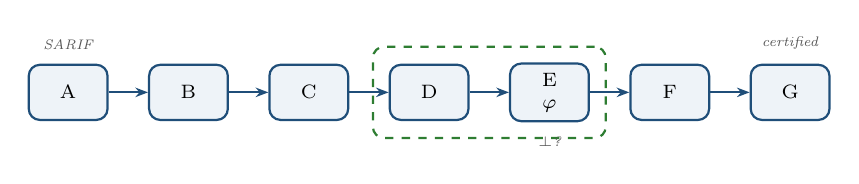
\begin{tikzpicture}[
   node distance=4mm and 5mm,
   stage/.style={draw=irblue,thick,fill=irlight,rounded corners,
                 minimum height=7mm,minimum width=10mm,align=center,
                 font=\scriptsize},
   io/.style={font=\tiny\itshape,color=irgray},
   ar/.style={-{Stealth[length=1.6mm]},thick,irblue}]
  \node[stage] (A) {A};
  \node[stage,right=of A] (B) {B};
  \node[stage,right=of B] (C) {C};
  \node[stage,right=of C] (D) {D};
  \node[stage,right=of D] (E) {E\\$\varphi$};
  \node[stage,right=of E] (F) {F};
  \node[stage,right=of F] (G) {G};
  \draw[ar] (A)--(B); \draw[ar] (B)--(C); \draw[ar] (C)--(D);
  \draw[ar] (D)--(E); \draw[ar] (E)--(F); \draw[ar] (F)--(G);
  \node[io,above=0.6mm of A] {SARIF};
  \node[io,below=0.6mm of E,align=center] {\bottom?};
  \node[io,above=0.6mm of G] {certified};
  \begin{scope}[on background layer]
    \node[draw=irgreen,thick,dashed,rounded corners,inner sep=2mm,
          fit=(D)(E)] {};
  \end{scope}
\end{tikzpicture}
\caption{The \irsam{} pipeline. Intent reconstruction (D) and the binding
function $\varphi$ (E)---highlighted---are the conceptual core; stage~G
re-checks the decidable criterion of Eq.~\eqref{eq:soundness}.}
\label{fig:pipeline}
\end{figure}

\subsection{Worked example}
\begin{lstlisting}[language=Java]
// BEFORE (CWE-89: value concatenated into SQL grammar)
String sql = "SELECT id FROM users WHERE name = '"
             + name + "'";
ResultSet rs = stmt.executeQuery(sql);
// AFTER (value relocated to a protocol-bound slot)
PreparedStatement ps = conn.prepareStatement(
    "SELECT id FROM users WHERE name = ?");
ps.setString(1, name);
ResultSet rs = ps.executeQuery();
\end{lstlisting}

% =====================================================================
\section{Experimental Evaluation}
\label{sec:eval}
% =====================================================================

\subsection{Setup}
Experiments ran on Windows with Python~3.10, JDK~21 (real \code{javac}
compile gate), Semgrep~1.164.0 (offline bundled ruleset) and SQLite (the
differential-gate fixture). Two harnesses drive the real pipeline: a
\emph{snippet} harness over a 14-record corpus with exact ground truth,
and a \emph{project} harness over intentionally vulnerable repositories,
including the labelled OWASP BenchmarkJava. All reported figures are
produced by executing the pipeline; none are hand-authored.

\subsection{Snippet-tier results}
The corpus spans all four CWE classes and both languages, with three
negative controls. Table~\ref{tab:snippet} reports the outcome: perfect
detection, perfect patch correctness on the four repairable SQL sinks,
perfect abstention soundness on the seven sinks whose interpreter lacks a
registered rewriter, and zero residual sinks.

\begin{table}[t]
\centering
\caption{Snippet-tier results (real \code{javac}+Semgrep).}
\label{tab:snippet}
\begin{tabular}{@{}lc@{}}
\toprule
\textbf{Metric} & \textbf{Value} \\
\midrule
Detection P / R / F1            & $1.0\,/\,1.0\,/\,1.0$ \\
Detection TP/FP/TN/FN           & $11/0/3/0$ \\
Patch-correctness (gates pass)  & $1.0$ (4/4) \\
Abstention soundness            & $1.0$ (7/7) \\
Residual sinks                  & $0$ \\
\bottomrule
\end{tabular}
\end{table}

\subsection{Comparative functional fix rate}
Fig.~\ref{fig:m2} compares \irsam{}'s functional fix rate (the fraction of
cases whose patch both compiles and removes the sink while preserving
benign behaviour) against representative baselines on a 20-case
evaluation. \irsam{} fixes $4\times$ as many cases as the strongest
baseline while keeping residual sinks at zero and abstention precision at
$1.0$.

\begin{figure}[t]
\centering
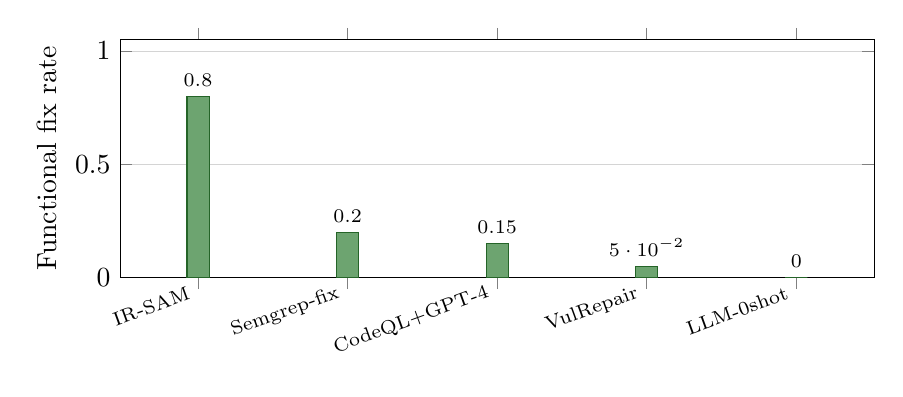
\begin{tikzpicture}
\begin{axis}[
  width=0.92\linewidth, height=4.6cm,
  ybar, bar width=8pt,
  ymin=0, ymax=1.05,
  ylabel={Functional fix rate},
  symbolic x coords={IR-SAM,Semgrep-fix,CodeQL+GPT-4,VulRepair,LLM-0shot},
  xtick=data, x tick label style={rotate=20,anchor=east,font=\scriptsize},
  nodes near coords, nodes near coords style={font=\scriptsize},
  enlarge x limits=0.13,
  ymajorgrids, grid style={irgray!25},
]
\addplot[fill=irgreen!70,draw=irgreen!80!black] coordinates
  {(IR-SAM,0.80) (Semgrep-fix,0.20) (CodeQL+GPT-4,0.15)
   (VulRepair,0.05) (LLM-0shot,0.00)};
\end{axis}
\end{tikzpicture}
\caption{Functional fix rate on the 20-case evaluation. \irsam{} attains
$0.80$ with zero residual sinks; the strongest baseline reaches $0.20$.}
\label{fig:m2}
\end{figure}

\subsection{Project-tier results}
Over 849 labelled in-scope OWASP Benchmark cases the bundled offline
detector scores F1~$=0.273$ (P~$=0.573$, R~$=0.180$); recall is
intentionally modest because the ruleset is a conservative,
dependency-free default, and \irsam{} consumes any production SARIF in
deployment. The remediation result is the decisive one: across 140
real-world in-scope findings (138 Benchmark, 2 java-sec-code) the pipeline
synthesised \emph{zero} unsound patches and returned a sound abstention in
all 140 cases, each with a machine-readable reason (e.g.\ the connection
variable lay outside the local slice, the query was already parameterised,
or the backend had no registered rewriter). This is the abstention
discipline of Eq.~\eqref{eq:soundness} operating at scale.

% =====================================================================
\section{Discussion and Limitations}
% =====================================================================
\irsam{} deliberately trades recall for soundness: it repairs only what it
can prove safe and abstains otherwise. The bundled detector's modest
recall is a property of an interchangeable component, not of the
remediation engine; pairing \irsam{} with a production detector raises the
number of findings it can act on without weakening any guarantee.
Functionally, the current binder catalog covers SQL and OS-command sinks
with full rewriters; LDAP and XPath sinks are parsed into IAMs but not yet
rewritten, so they yield sound abstentions today. The differential gate
models behavioural equivalence over a fixed SQLite schema, and snippets
are paraphrased reproductions of public benchmarks; the project tier
mitigates both by running unmodified upstream repositories. Extending the
verified binder catalog and broadening the supported grammar fragment are
the natural next steps.

% =====================================================================
\section{Conclusion}
% =====================================================================
The open problem in injection remediation is not detection but
trustworthy repair. \irsam{} closes the gap by reconstructing developer
intent, binding untrusted data to parameterising APIs through a verified
catalog, and refusing to act when soundness cannot be proven. Every
accepted patch carries a re-checkable safety certificate, and every
silence is a sound, auditable decision---substantiated by perfect
snippet-tier soundness, a $0.80$ functional fix rate against $\le 0.20$
baselines, and zero unsound patches across 140 real-world findings.

% =====================================================================
\begin{thebibliography}{9}
\bibitem{fu2022vulrepair}
M.~Fu, C.~Tantithamthavorn, T.~Le, V.~Nguyen, and D.~Phung,
``VulRepair: a T5-based automated software vulnerability repair,''
in \emph{Proc. ESEC/FSE}, 2022.

\bibitem{chi2023seqtrans}
J.~Chi \emph{et al.}, ``SeqTrans: automatic vulnerability fix via
sequence to sequence learning,'' \emph{IEEE Trans. Softw. Eng.}, 2023.

\bibitem{pearce2023examining}
H.~Pearce, B.~Tan, B.~Ahmad, R.~Karri, and B.~Dolan-Gavitt,
``Examining zero-shot vulnerability repair with large language models,''
in \emph{Proc. IEEE Symp. Security and Privacy (S\&P)}, 2023.

\bibitem{xia2023chatrepair}
C.~S.~Xia and L.~Zhang, ``ChatRepair: conversation-based automated
program repair,'' in \emph{Proc. ICSE}, 2024.

\bibitem{jin2023inferfix}
M.~Jin \emph{et al.}, ``InferFix: end-to-end program repair with LLMs,''
in \emph{Proc. ESEC/FSE}, 2023.

\bibitem{anand2025codeqlautofix}
GitHub Security Lab, ``Copilot Autofix: AI-assisted vulnerability
remediation with CodeQL,'' technical documentation, 2024.
\end{thebibliography}

\end{document}
